\documentclass{article}
\usepackage[a4paper,scale=0.8,hcentering,bindingoffset=8mm]{geometry} % A4纸大小,缩放80%,设置奇数页右边留空多一点
\usepackage{hyperref}      % 超链接
\usepackage{listings}      % 代码块
\usepackage{courier}       % 字体
\usepackage{fontspec}      % 字体
\usepackage{fancyhdr}      % 页眉页脚相关宏包
\usepackage{lastpage}      % 引用最后一页
\usepackage{amsmath,amsthm,amsfonts,amssymb,bm} %数学
\usepackage{graphicx}      % 图片
\usepackage{subcaption}    % 图片描述
\usepackage{longtable,booktabs} % 表格
\usepackage{ctex}
\usepackage{soul}
\usepackage{dot2texi}
\usepackage{tikz}
\usepackage{multirow}
\usepackage{float}
% \setmainfont{Noto Sans Kaithi}
\usetikzlibrary{automata, positioning, arrows}
\lstset{                  %设置代码块
         basicstyle=\footnotesize\ttfamily,% 基本风格
         numbers=left,    % 行号
         numbersep=10pt,  % 行号间隔 
         tabsize=4,       % 缩进
         extendedchars=true, % 扩展符号?
         breaklines=true, % 自动换行
         language=C,
         frame=leftline,  % 框架左边竖线
         xleftmargin=5pt,% 竖线左边间距
         showspaces=false,% 空格字符加下划线
         showstringspaces=false,% 字符串中的空格加下划线
         showtabs=false,  % 字符串中的tab加下划线
 }
\pagestyle{fancy}         % 页眉页脚风格
\fancyhf{}                % 清空当前设置
\fancyfoot[C]{\thepage\ / \pageref{LastPage}}%页脚中间显示 当前页 / 总页数,把\label{LastPage}放在最后
\begin{document} 
    \begin{titlepage}       % 封面
        \centering
        
\includegraphics[width=\textwidth]{../SUSTC_LOGO.png}
        % \vspace*{\baselineskip}
        \rule{\textwidth}{1.6pt}\vspace*{-\baselineskip}\vspace*{2pt}
        \rule{\textwidth}{0.4pt}\\[\baselineskip]
        {\LARGE COMPILIER @Liu Yepang 2019\\[\baselineskip]\small for SUSTech CSE}
        \\[0.2\baselineskip]
        \rule{\textwidth}{0.4pt}\vspace*{-\baselineskip}\vspace{3.2pt}
        \rule{\textwidth}{1.6pt}\\[\baselineskip]
        \scshape
        \vspace*{\baselineskip}
        {\Large HomeWork 4\par }
        Edited by \\[\baselineskip] {汪至圆\par}
        {\Large 11610634\par }
        \vfill
        {\scshape 2019} \\{\large SHENZHEN}\par
    \end{titlepage}
    \section{Exercise 1: For the SDD in Figure 1, give annotated parse trees for the following expressions:}
        \begin{figure}[H]
            \centering
            \caption{Syntax-directed definition of a simple desk calculator}
            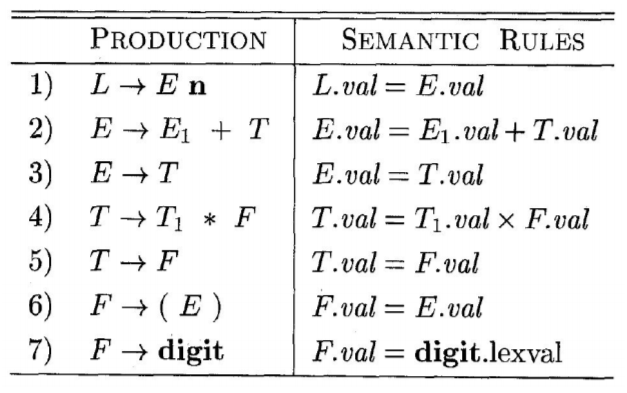
\includegraphics[scale=0.5]{./Q1_T.png}
            \label{fig:label}
        \end{figure}
        \subsection{(3 + 4) ∗ (5 + 6)n [20 points]}
        \begin{figure}[H]
            \centering
            
            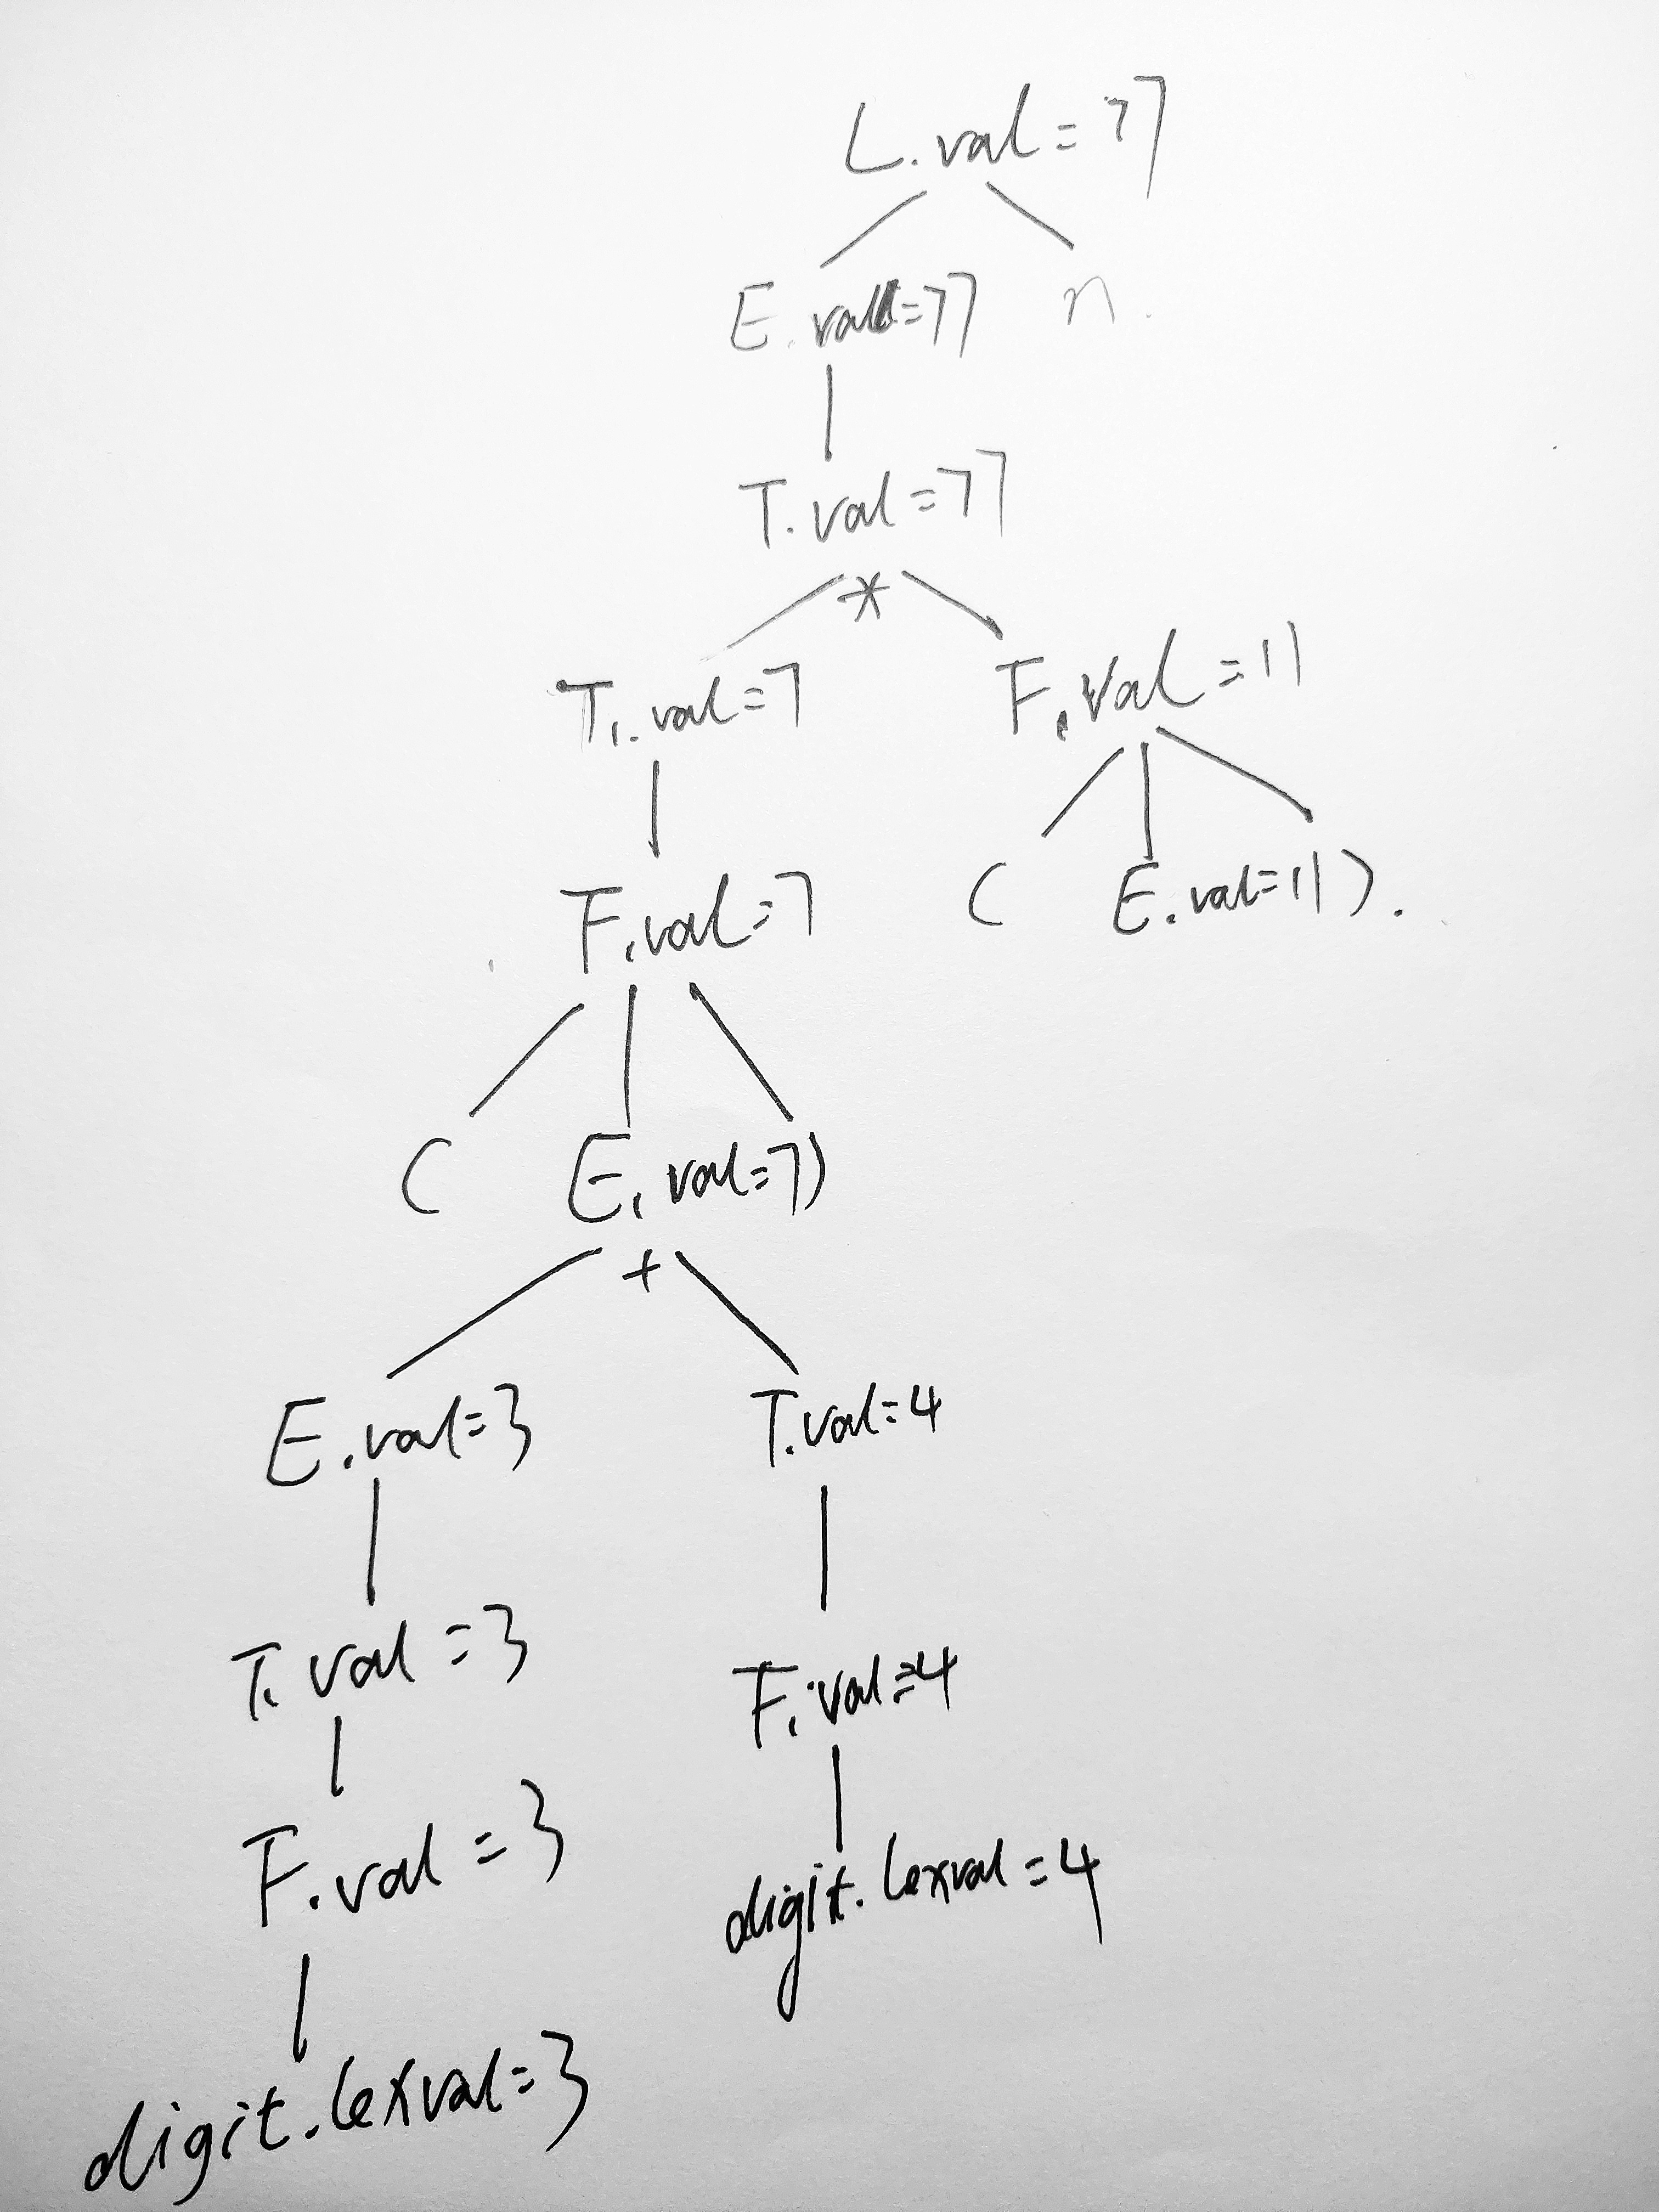
\includegraphics[scale=0.15]{./Q1_1.jpg}
            \label{fig:label}
        \end{figure}
        \subsection{1 ∗ 2 ∗ 3 ∗ (4 + 5)n [20 points]}
        \begin{figure}[H]
            \centering
            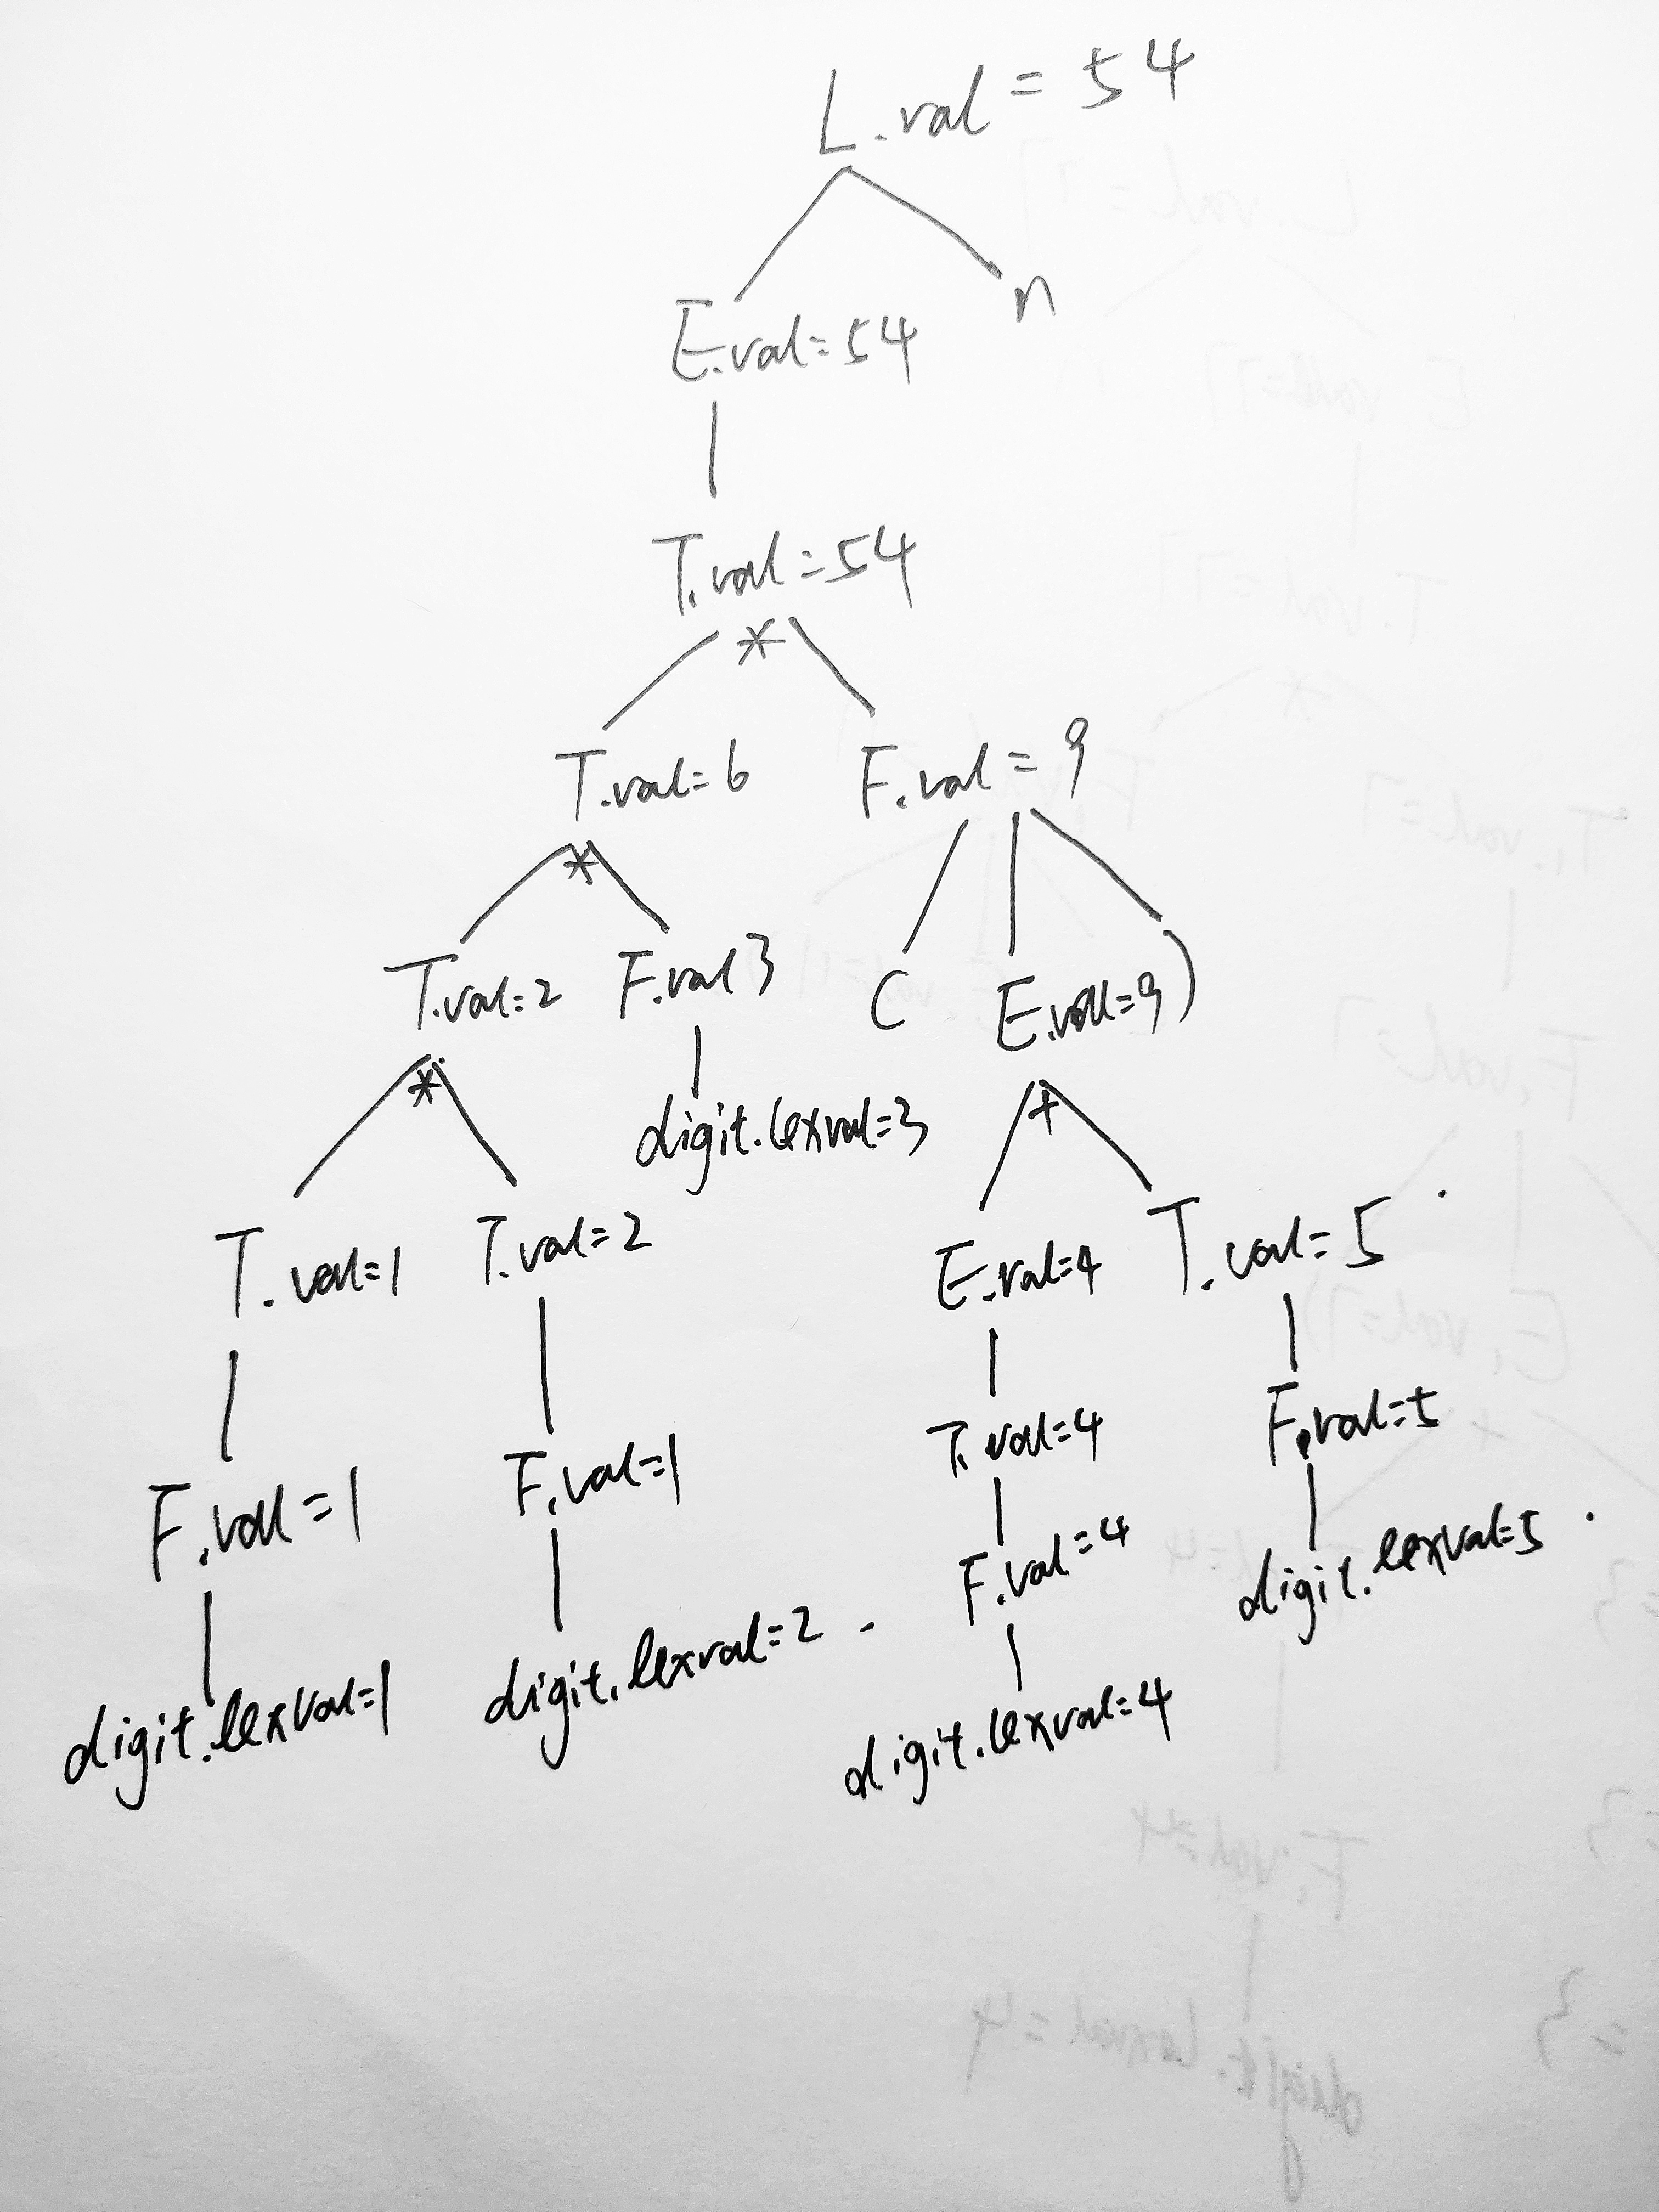
\includegraphics[scale=0.15]{./Q1_2.jpg}
            \label{fig:label}
        \end{figure}
        \subsection{(9 + 8 ∗ (7 + 6) + 5) ∗ 4n [20 points]}
        \begin{figure}[H]
            \centering
            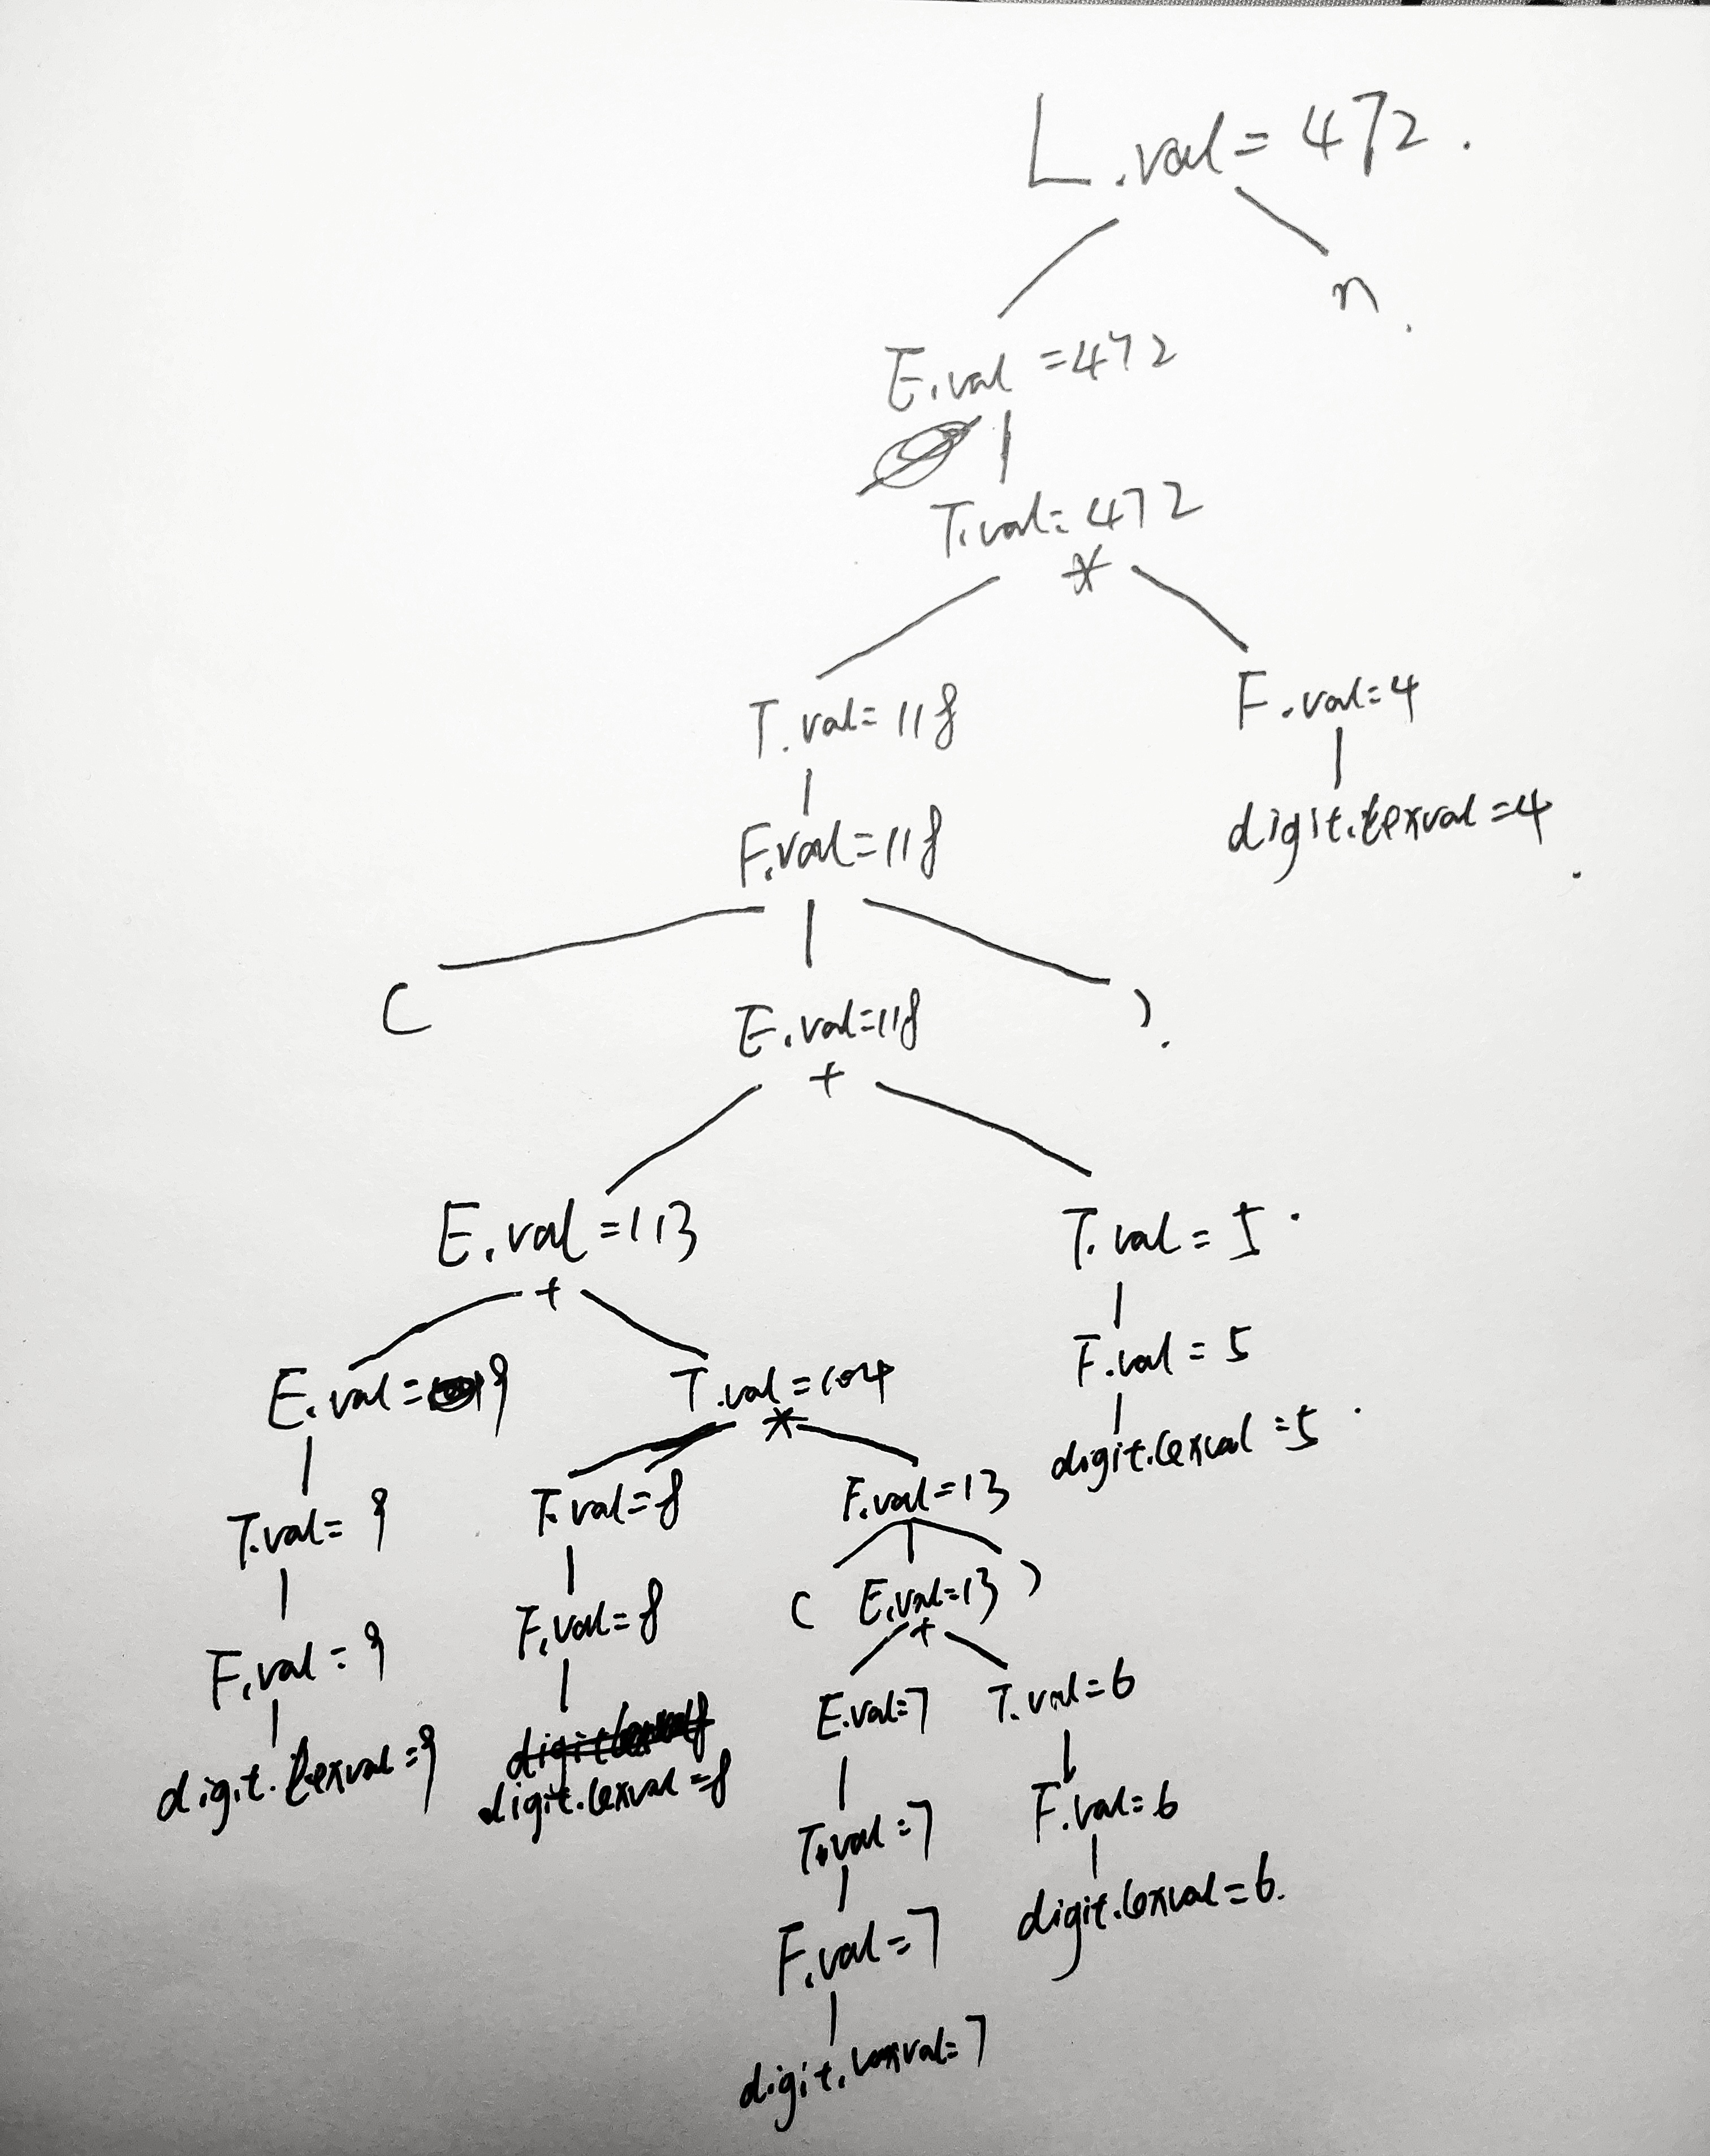
\includegraphics[scale=0.15]{./Q1_3.jpg}
            \label{fig:label}
        \end{figure}
    \section{Exercise 2: What are all the topological sorts for the dependency graph of Figure 2? One 
    sort mentioned during lecture is 1, 2, 3, . . . , 9 (slide \#16 of Chapter 4). [20 points]}
        \begin{figure}[H]
            \centering
            \caption{A dependency graph}
            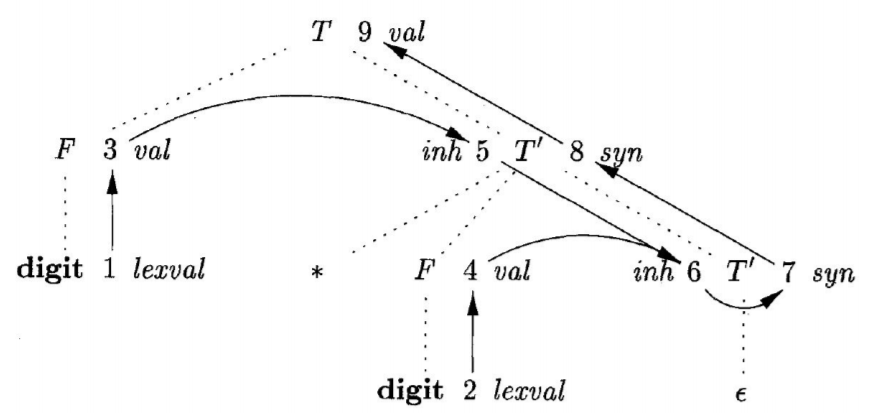
\includegraphics[scale=0.5]{./Q2_T.png}
            \label{fig:label}
        \end{figure}
        The sequence must end with 6,7,8,9 and it can start with 1 or 2. So all the topological sorts of the dependency 
        graph is:
        \begin{itemize}
            \item 2,4,1,3,5,6,7,8,9
            \item 2,1,4,3,5,6,7,8,9
            \item 2,1,3,4,5,6,7,8,9
            \item 2,1,3,5,4,6,7,8,9
            \item 1,2,4,3,5,6,7,8,9
            \item 1,2,3,4,5,6,7,8,9
            \item 1,2,3,5,4,6,7,8,9
            \item 1,3,2,4,5,6,7,8,9
            \item 1,3,2,5,4,6,7,8,9
            \item 1,3,5,2,4,6,7,8,9
        \end{itemize}
    \section{Exercise 3: Below is a grammar for expressions involving operator + and integer or floatingpoint operands. Floating-point numbers are distinguished by having a decimal point. Give
    an SDD to determine the type of each term T and expression E. [20 points]}
    $$
        \begin{aligned} E \rightarrow E+T | T \\ T \rightarrow \operatorname{num} \cdot \operatorname{num} | \operatorname{num} \end{aligned}
    $$
    \begin{table}[!htbp]
        \centering
        \label{tab:aStrangeTable}
        \begin{tabular}{|c|c|}
            \hline
            $E\rightarrow E_1+T$ & $E.type = (E_1.type == float||T.type ==float)?float:int$\\
            \hline
            $E\rightarrow T$ & $E.type = T.type$ \\
            \hline
            $T\rightarrow num.num$ & $T.type = float$\\
            \hline
            $T->num$ & $T.type = int$\\
            \hline
            
        \end{tabular}
    \end{table}
    
\end{document}